
\subsection{Faraday-Effekt}
\subsubsection*{Bestimmung der Verdetkonstante}
Um die Verdetkonstante zu berechnen, haben wir die Rotation des Lichtes welches durch ein Schwerflintglas in einer Spule verlief, in Abhängigkeit des Magnetfelds der Spule gemessen.
\begin{figure}[h]
\begin{center}
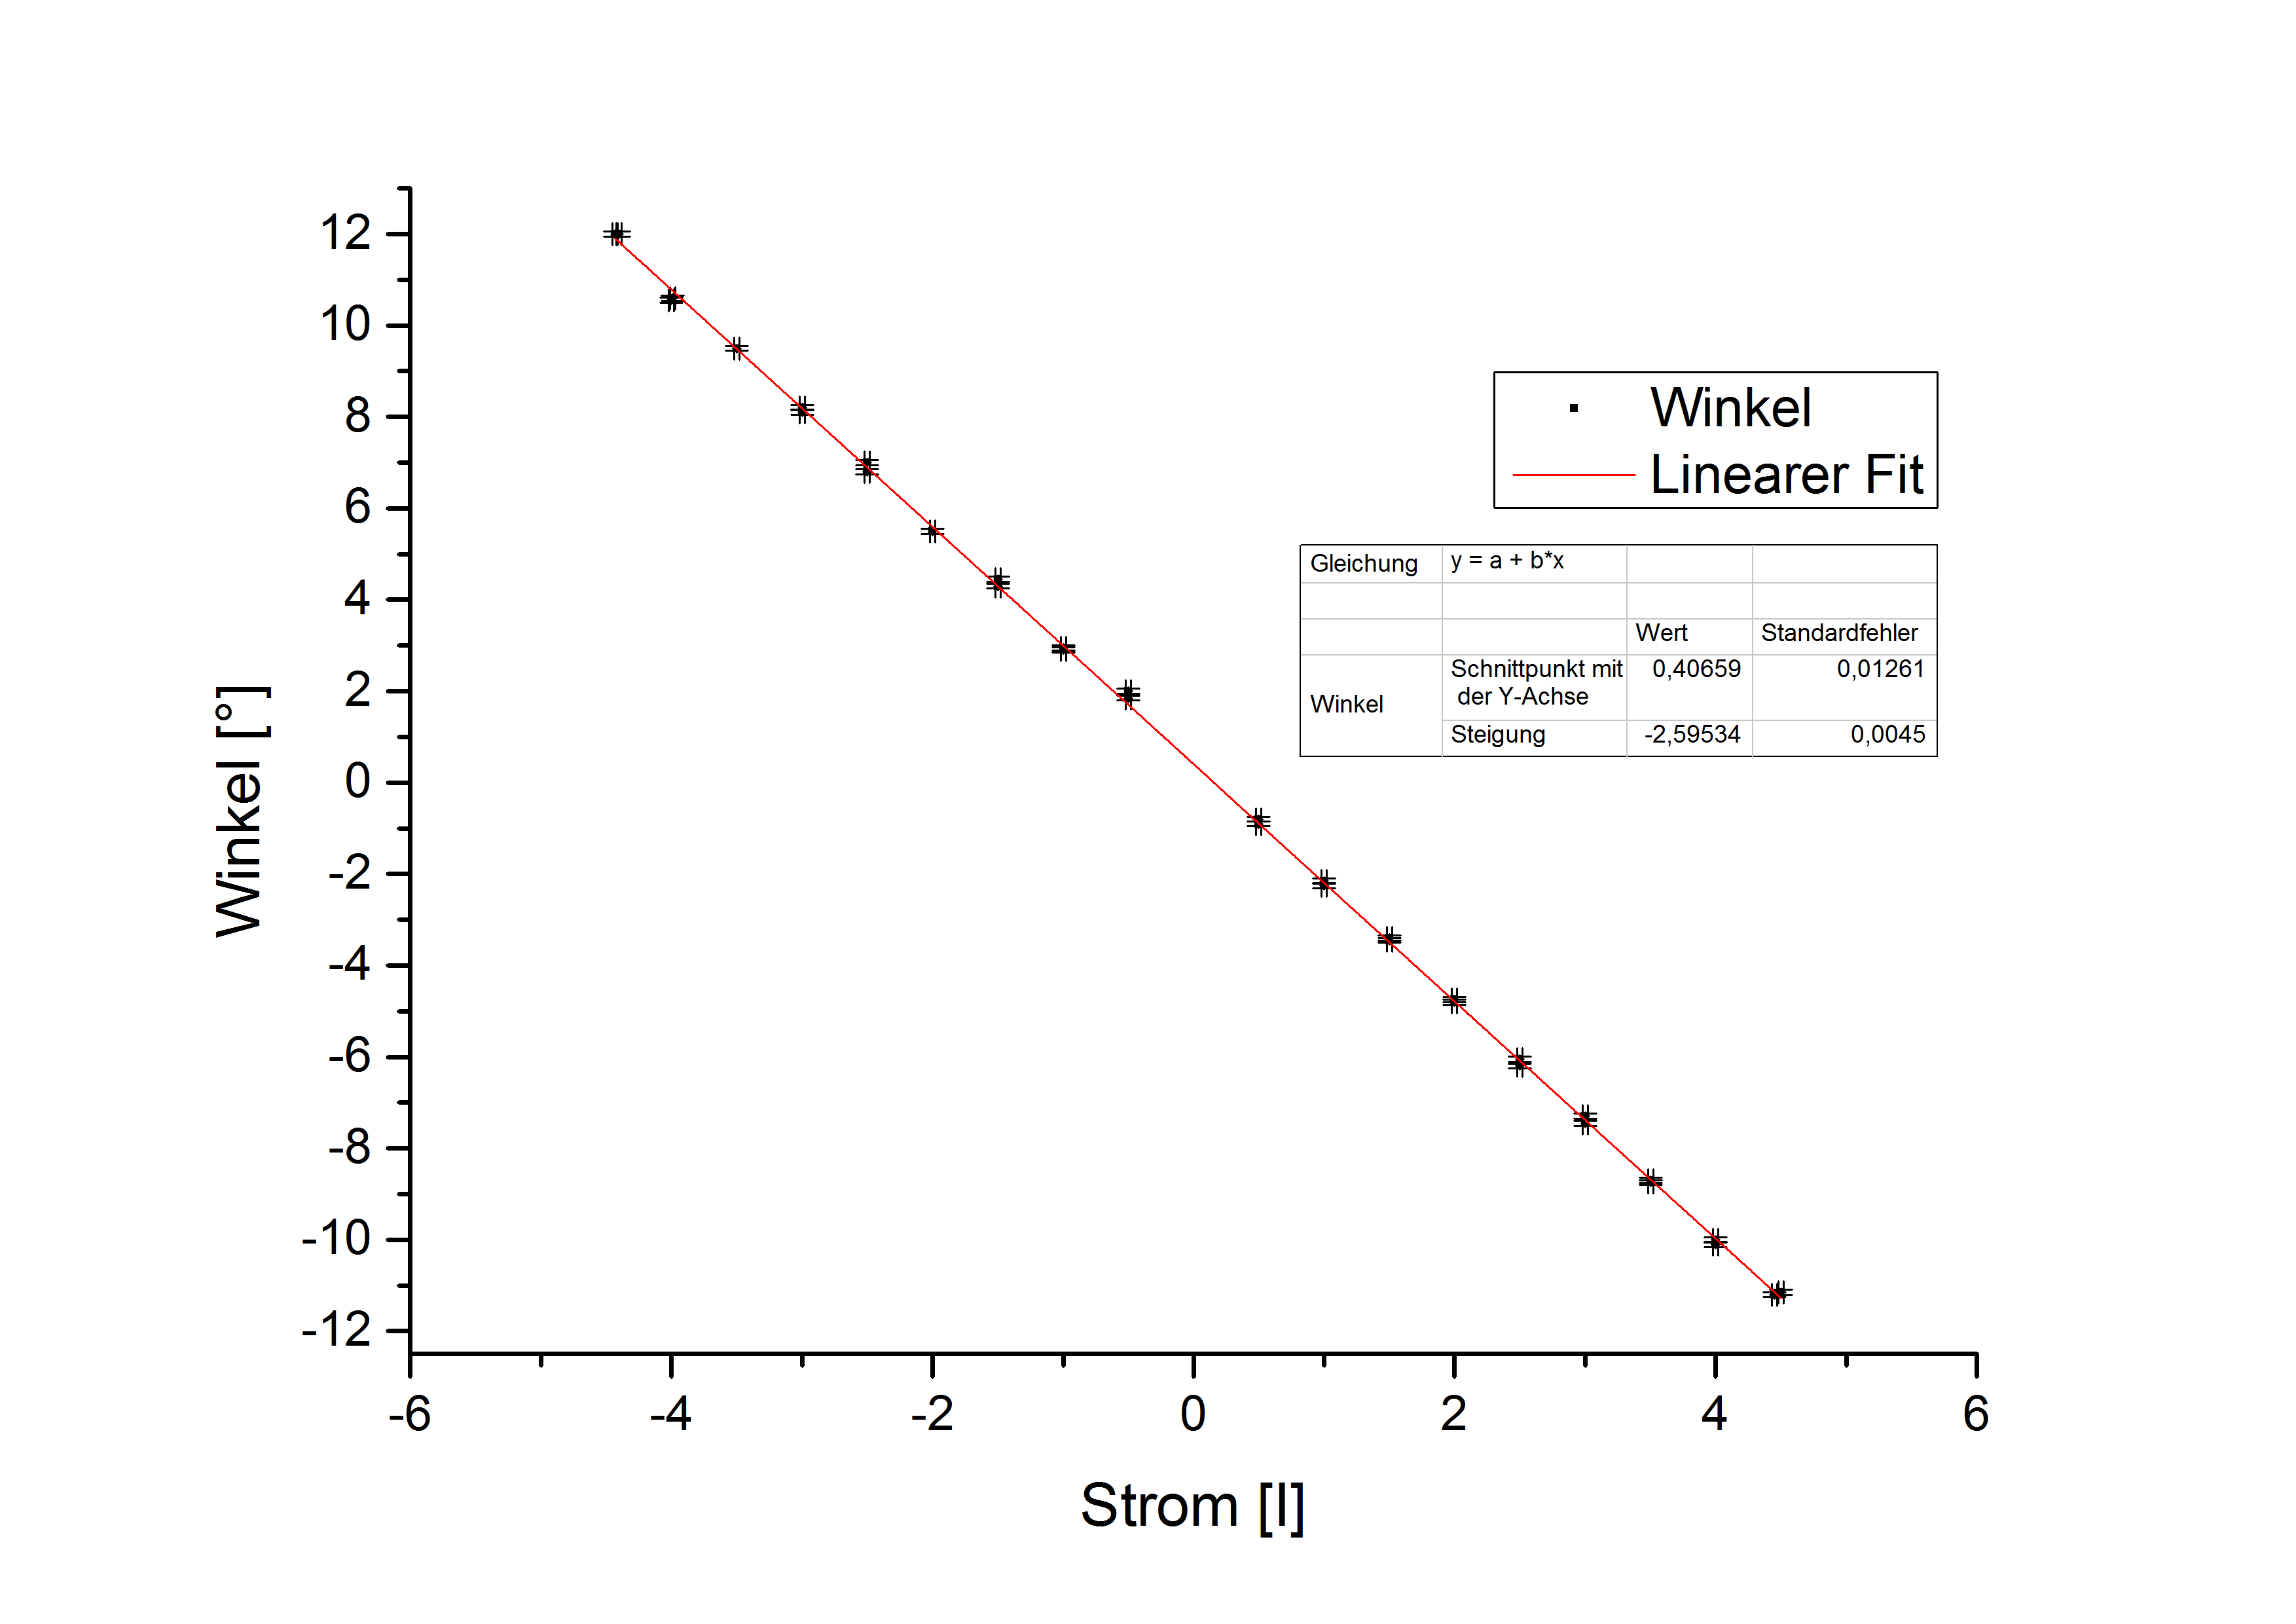
\includegraphics[scale=0.3]{faraday_lin}
\caption{Linearer Fit beim auftragen von Winkel über Stromstärke}
\label{fig:faraday_lin}
\end{center}
\end{figure}
~\\
Die Ableseungenauigkeit auf die Winkel haben wir durch eine gesonderte Messung zu beginn des Versuches bestimmt, siehe Anhang. Hierbei haben wir bei der selben Spannung Mehrfach den Winkel abgelesen, bei denen das Halbschattenpolarimeter innen und außen die selbe Intensität aufweist. Da der korrekte Winkel nicht vorlag können wir keine Personenbezogene Wichtung vornehmen. Als Fehler auf die Messung des Winkels in den weiteren Versuchsteilen haben wir, dadurch die Standardabweichung der Einzelwerte benutzt, diese beträgt $s_\alpha = 0,06\,^{\circ} $.\\
Um das Verhältnis von Stromstärke $I$ und der magnetischen Feldstärke $H$ der Spule zu erhalten benutzen wir das Biot-Savart-Gesetz. Die Herleitung und Berechnung der magnetischen Feldstärke kann in der Arbeit von Bernd Herrman ("Elektrooptischer Effekt und Faraday Effekt") nachgeschlagen werden.
\begin{center}
\[ d\alpha = V \cdot H(z)\cdot dz  \Rightarrow \alpha = 2556 \cdot V \cdot I\]
\[ V = \frac{\alpha}{2556 \cdot I}\]
\end{center}
Hierbei ist $\alpha$ der Winkel um welches sich dir Polarität gedreht hat, $V$ ist die Verdetkonstante und $I$ die Stromstärke. Aus dem linearen Fit oben lässt sich die Steigung $b$ auslesen. Diese entspricht genau dem Verhältnis aus:
\[b = \frac{Winkel}{Stromstärke}=\frac{\alpha}{I}\]
\[\Rightarrow V=\frac{b}{2556}\]
Wenn wir nun von Grad-maß zu Radiant wechseln erhalten wir:
\begin{center}
\[V=b \cdot \frac{3979}{213} \cdot 10^{-3} \frac{min}{Oe ~ cm} \]
\end{center}
Der Fehler auf $V$ ergibt sich aus:
\begin{center}
\[s_{V}= V \cdot \frac{s_b}{b}\]
\end{center}
Die Verdetkonstante für Schwerflintglas und die Wellenlänge des Lichtes der Natriumdampflampe von $\lambda = 589 nm$, beträgt:
\begin{center}
\[ V_{SF,589}=(-0,04848\pm0,00008) \frac{Min}{Oe~cm} \]
\end{center}

~\\
\subsubsection*{$2 \epsilon$ Messung}
Nun haben wir zum vermessen des Winkels $\beta$ um welchen die Polarisationsrichtungen des Halbschattenpolarimeters verschoben sind, jeweils den Winkel der beiden Hälften vermessen bei denen sie jeweils am dunkelsten sind. Die Messwerte hierfür befinden sich im Anhang. Aus den zwei Werten wurde jeweils der Mittelwert berechnet.\\
Man erhält also:\\
\[ \alpha_{1,J}=9,15\,^{\circ} ,~~~~~~~~~~~ \alpha_{1,D}=8,10\,^{\circ} \]
\[ \Rightarrow \alpha_1 = (8,63\pm0,04)\,^{\circ} \]
\[ \alpha_{2,J}=171,4\,^{\circ} ,~~~~~~~~~~~ \alpha_{2,D}=175,4\,^{\circ} \]
\[ \Rightarrow \alpha_1 = (173,4\pm0,04)\,^{\circ} .\]
Der Fehler folgt aus der oben genannten Fehlermessung.
Für die $2\epsilon$ Messung gilt nun:
\[ 2\epsilon = \mid \alpha_1 - \alpha_2 \mid = (164,77\pm0,06)\,^{\circ} \]
Der Fehler berechnet sich aus $s_{2\epsilon}=\sqrt{2} \cdot s_{\alpha_1}$, da die beiden Fehler auch hier als gleich angenommen werden müssen.\\
Die großen Unterschiede der obigen $2\epsilon$-Messung könnte daran liegen, dass einer von uns oder beide die zu vermessende Stelle nicht richtig getroffen hat. Da wir auch hier keinen Literatur-/Eichwerte kennen, sind die Messergebnisse gleich gewichtet. Da wir wissen, dass die Maximalstellen mit bloßem Auge schlecht zu bestimmen sind liegt es nahe, dass der statistische Fehler hier zu klein ist.